\chapter{Geometry and Trigonometry}
\thispagestyle{fancy}

\keyword{Geometry} is a branch of mathematics that deals with the study of shapes, sizes, positions, and properties of space. It explores the relationships and properties of points, lines, angles, surfaces, and solids. In geometry, fundamental concepts include:

\begin{enumerate}
	\item \keyword{Points}: Basic building blocks with no size or dimensions. They are represented by dots and are used to define other geometric elements.
	\item \keyword{Lines}: Straight paths that extend infinitely in both directions. They are made up of an infinite number of points.
	\item \keyword{Angles}: The measure of the rotation between two intersecting lines, rays, or line segments.
	\item \keyword{Polygons}: Closed figures formed by connecting line segments to create shapes like triangles, quadrilaterals, pentagons, etc.
	\item \keyword{Circles}: A set of points equidistant from a central point, forming a closed curve.
	\item \keyword{Three-dimensional shapes}: Solids such as cubes, spheres, cylinders, pyramids, etc., with length, width, and height.
	\item Higher-dimensional shapes or objects: In addition to the traditional two-dimensional and three-dimensional shapes, geometry also explores mathematical constructs extended to higher dimensions. These higher dimensions go beyond our familiar three-dimensional space and introduce concepts like 4D, 5D, and higher-dimensional shapes. For example, in 4D space, there could be hypercubes, 4D spheres, and other intriguing structures. While challenging to visualize, these higher-dimensional geometries play a crucial role in theoretical mathematics and various scientific fields, offering unique insights into the nature of space and dimensions beyond our immediate perception.
\end{enumerate}

Geometry plays a significant role in various fields, including architecture, engineering, art, design, physics, and many other disciplines. It helps us understand the physical world and solve problems related to spatial relationships and measurements. Euclidean geometry, founded by the ancient Greek mathematician Euclid, is one of the most well-known and widely studied branches of geometry. However, there are also other types of geometries, such as non-Euclidean geometries, which explore different axioms and concepts, leading to intriguing and diverse mathematical systems.




\section{Triangles}


\begin{defn}[The Law Of Cosines \label{defn:Law Of Cosines}]{1}
\keyword{The Law of Cosines} relates the side lengths of a triangle to the cosine of one of its angles. For a triangle with side lengths $a$, $b$, and $c$, and angle $C$ opposite to side $c$, the Law of Cosines is given by:
\begin{center}
\begin{minipage}{0.3\linewidth}
	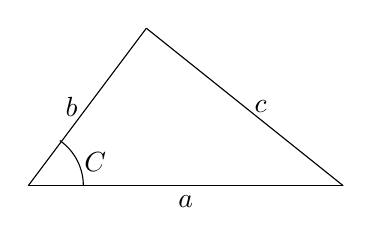
\begin{tikzpicture}
		% Triangle vertices
		\coordinate (A) at (0,0);
		\coordinate (B) at (4,0);
		\coordinate (C) at (1.5,2);
		
		% Triangle sides
		\draw (A) -- (B) node[midway,below] {$a$};
		\draw (B) -- (C) node[midway,right] {$c$};
		\draw (C) -- (A) node[midway,left] {$b$};
		
		% Angle C
		\draw (0.7,0) arc (0:55:0.7);
		\node at (0.85,0.3) {$C$};
	\end{tikzpicture}
\end{minipage}
\begin{minipage}{0.4\linewidth}
	\begin{align}
		c^2 = a^2 + b^2 - 2ab\cos C
	\end{align}
\end{minipage}
\end{center}
\end{defn}

Notice from definition \ref{defn:Law Of Cosines} that if the angle $C = 90^\circ = \pi/2$, then the cosine term would evaluate to zero and we'd be left with \keyword{the Pythagorean theorem} $c^2 = a^2 + b^2$.
